\documentclass[a4paper, 12pt]{report}
\renewcommand{\tiny}{\normalsize}
\renewcommand{\footnotesize}{\normalsize}
%\renewcommand{\small}{\normalsize}
%\renewcommand{\large}{\normalsize}
%\renewcommand{\Large}{\normalsize}
%\renewcommand{\LARGE}{\normalsize}
%\renewcommand{\huge}{\normalsize}
%\renewcommand{\Huge}{\normalsize}
\usepackage{fancyhdr,blindtext}
\pagestyle{fancy}
\usepackage{enumitem}
\usepackage{graphicx} 
\usepackage{caption} 
\usepackage{subcaption} 
\usepackage{parskip}
\setlength{\parindent}{15pt}
\usepackage[margin=0.75in]{geometry}
\usepackage{listings}
\usepackage{amsmath}
\usepackage{hyperref}



\lstset{
	frame=single,
	breaklines=true
	columns=flexible
	keepspaces=true
}
\lstdefinestyle{myCustomPythonStyle}{
	language=R,
	numbers=left,
	stepnumber=1,
	numbersep=10pt,
	tabsize=5,
	showspaces=false,
	showstringspaces=false
}


\begin{document}
\begin{titlepage}
	\centering
	{\scshape\LARGE University of California, Davis \par}
	{\scshape\Large STA160 Project Report\par}
	\vspace{5cm}
	
	
	{\huge\bfseries Identify Fake Users on Twitter \par}
	\vspace{3cm}
	
	{\Large Guanyu Chen \par}
	{\large\itshape SID: 999329481 \par}
	
	{\Large Jieyi Chen \par}
	{\large\itshape SID: \par}

	{\Large Tongke Wu\par}
	{\large\itshape SID:914478812 \par}
		\vfill
% Bottom of the page
	{\large \today\par}
\end{titlepage}

\section*{ABSTRACT}
Social networks, such as Twitter, have become a popular tool to interact with people and spread news. However, there are large amount of fake/spam users generating useless even malicious information. Therefore, it is an essential and challenging work to detect the fake/spam accounts and maintain imformative social networking. \par

\noindent In this project, we use 47 features to depict behavior of Twitter users especially fake/spam accounts and develop random forest, logistic regression and support vector machine models based on these information to discriminate fake/spam accounts from genuine users. 
\section*{INTRODUCTION}
As Twitter rapidly grows, a great number of fake/spam accounts infiltrate into social networking. According to the study conducted by the University of Southern California and Indiana University\footnote{O.Varol, E.Ferrara, C.A.Davis, F.Menczer, and A.Flammini. Online Human-Bot Interactions: Detection, Estimation, and Characterization}, there are approximately 9 - 15\% Twitter active monthly users are bots, which are around 28.9 million to 47.9 million potential fake users. We believe there are three negative effects brought by those fake/spam accounts.
\begin{enumerate}
	\item \textbf{Misleading propagand:} it includes misleading infromation related to certain news and falsely boosted popularity of users  Twitter users might become less interested when they go through a great deal of fraudulent information.
	\item \textbf{Fishing information:} it is maily about malicious urls which redirect users to fishing websites. Users would suffer from the leak of private information and financial losses if they are exposed to fishing urls.
	\item \textbf{Intrusive advertisement:} it would reduce the advertisement income for Twitter if entities use cheap computer-generated bots to promote products.
\end{enumerate}
Therefore, effective detection of fake accounts will help Twitter to purify the online communities and improve user experience. Meanwhile, it could prevents Twitter from loosing advertisement business share as well.

\section*{DATA}
\subsection*{Sourse}
\textbf{Labeled Twitter User Account:} to construct a diverse dataset, we have four kinds of Twitter user accounts:
\begin{enumerate}
	\item Genuine users: verified accounts that are human-operated
	\item Social spambots: retweeters of an Italian political candidate, spammers of paid apps for mobile devices and spammers of products on sale at Amazon.com
	\item Traditional spambots: training set of spammers used by C. Yang, R. Harkreader, and G. Gu \footnote{C. Yang, R. Harkreader, and G. Gu. Empirical evaluation and new design for fighting evolving Twitter spammers. I.}, spammers of scam URLs, automated accounts spamming job offers, another group of automated accounts spamming job offers	
	\item Fake users: simple accounts that inflate the number of followers of another account
\end{enumerate}
Among them, genuine users, social spambots and traditional spambots are acquired from \href{http://mib.projects.iit.cnr.it/dataset.html}{My Information Bubble}. Fake users are provided by \href{https://www.fastfollowerz.com/closed/}{Fast Followerz}'s paid service. \par

\noindent\textbf{Tweets and Users' Profile Data:} we used user id's provided by the labeled Twitter user account data to require latest users' profile, tweets and followers/followings information from Twitter API.

\subsection*{Limitation}
\begin{enumerate}
	\item The fake accounts provided by MIB are related to specific topics like retweeters of an Italian political candidate. Then these accounts may share similar contents and charactristics.
	\item We were limited to Twitter API's rate limits where we can only make certain number of requests per 15 minute periods. Unfortunately, the number of successful requests kept decreasing as we requsted more data. And there exsits the situation that Twitter API dose not return all the infromatin we require. In addition, we can only retrieve a maximum of 3,200 possible tweets for one user. 
\end{enumerate}

\section*{METHODOLOGIES}
\subsection*{Feature Engineering}
Although Twitter makes efforts to filter fake/spam users out, fake accounts and spammers are still evolving and developing tactics to evade existing detection techniques. It is important and challenging to apply appropriate features to capture the patterns of behavior of fake users. \par

\noindent Fake users and spammers tend to follow a large number of people who are probably irrelevant. For imformation spreading purpose, such as advertisement spam bots, they are likely to post tweets with high frequency and similar content. Therefore, besides basic data from Twitter API, we need to further processing of them to generate effective features to depict fake users' behavior.

\subsection*{Classifiers}
\subsubsection*{Random Forest Tree}
Random Forest is a supervised machine learning technique for classification and regression. In this project, we will specifically use it to perform classification tasks because  we want to predict whether the twitter account is genuine or fake. \par

\noindent As for advantages, Random Forest is one of the most accurate classifier available which can perform well even with missing or unbalanced datasets. It can accurately identify the important variables without deletion even with thousands of input variables. And we can get the importances of predictive variables in the model. \par

\noindent However, Random Forest might over-fit the datasets. And it might be biased toward categorical variables with different number of levels. Unlike other models, we have very little control of the model because we can only tune the parameters and the random seeds.

\subsubsection*{Logistic Regression}
Logistic regression belongs to the family of classifiers known as the exponential or log-linear classifiers. It works by extracting some set of weighted features from the input, taking logs, and combining them linearly (meaning that each feature is multiplied by a weight and then added up). Technically, logistic regression refers to a classifier that classifies an observation into one of two classes, and multinomial logistic regression is used when classifying into more than two classes, although informally we sometimes use the shorthand logistic regression even when we are talking about multiple classes.\par

\noindent If a feature is perfectly predictive of the outcome because it happens to only occur in one class, it will be assigned a very high weight. The weights for features will attempt to perfectly fit details of the training set, in fact too perfectly, modeling noisy factors that just accidentally correlate with the class. This problem is called \textbf{overfitting}.

\noindent Therefore, there are two common regularization terms called **L1** and **L2** to avoid overfitting:

\noindent \textbf{L1} regularization is a linear function of the weight values, named after the L1 norm $|w|$, the sum of the absolute values of the weights. \\
\textbf{L2} regularization is called ridge regression which is sum of the square of the weights $||w||$.

\noindent\textbf{The LogisticRegression in sklearn:}
Logistic regression is also known in the literature as logit regression, maximum-entropy classification (MaxEnt) or the log-linear classifier. In this model, the probabilities describing the possible outcomes of a single trial are modeled using a \href{https://en.wikipedia.org/wiki/Logistic_function}{logistic function} \par

\noindent To opimize the problem, we need to minimize the 

$$
f(x) = \frac 1 {1+e^{-x}}
$$

\noindent L1 regularized logistic regression solves the following optimization problem:
$$
min\frac1{2}w^Tw + C \sum_{i = 1}^n log(exp(-y_{i}(X_{i}^Tw + c)) + 1)
$$

\noindent L2 penalized logistic regression minimizes the following cost function:

$$
min\frac1{2}||w||_{1} + C \sum_{i = 1}^n log(exp(-y_{i}(X_{i}^Tw + c)) + 1)
$$

\subsubsection*{Support Vector Machine}
As ordinary discriminative classifiers, Support Vector Machine
takes in labeled training data and then outputs an optimal hyperplane which categorizes new examples. Especially for nonseperatable case, SVM is able to draw nonlinear boundary among classes. It aims to optimize
$$min_{\beta, \beta_0}\frac{1}{2}||\beta||^2+C\sum_{i=1}^{N}\xi_i$$ 
$$subject\ to\ \xi_i\geq 0,\ y_i(x_i^T\beta+\beta_0)\geq 1-\xi_i\ \forall i$$ 
where $C$ is the penalty/cost, $\xi_i$ are slack variables. The value $xi_i$ in the constraint is the proportional amount by which the prediction $f(x_i)=x_i^T\beta+\beta_0$ is on the wrong side of its margin.\\
SVM is robust in high dimensional sapces and can still work when the demension of features is larger than the sample size. In addition, different kernal functions can be assigned to the desicion funtion so that nonlinear relation can be satisfied.\\
In our project, we used rbf kernel and linear kernel as following
\begin{enumerate}
	\item []linear:\ $<x,x^{'}>$
	\item []rbf:\ $exp(-\gamma|x-x^{'}|^2)$
\end{enumerate}

\section*{ANALYSIS}
In order to approach the approximate proportion of fake/spam users in reality, we made our sample data 10.78\% of which are fake users selected randomly. And then We generated 3 sample data for futher validation purpose.
\subsection*{Feature Exploration}
Inspered by exsisting papers, we adopted 47 features categorized into profile features, content features, behavior features and graph features. \par

\noindent We selected several important features to make detailed explaination. \par

\noindent\textbf{Fo-Fo ratio:} Fo-Fo ratio is the number of an account's following to its followers. Since a bot is not a real person; thus, nobody knows him/her in real life, only a fraction of the profiles contacted would acknowledge a friend request. Also, one would expect a distinct difference between the number of friend requests sent and the number of those that are acknowledged. More precisely, we expect the ratio of friend requests to actual friends to be large for spammers and low for regular users (where following, in the Twitter jargon, is the number of friend requests sent, and followers is the number of users who accepted the request).

\noindent\textbf{Tweeting rate:} Tweeting rate is the ratio of number of tweets for a user to the total dates for tweeting. Since a bot might post many duplicate tweets in short time to get notices from other people , thus it has a relative higher tweet rate. Generally, normal users would not prefer to twittering very frequently and thus has lower tweet rate.

\noindent\textbf{Tweeting time:} We calculated the time interval between two consecutive tweets and conducted a basic summary statistics. Fake users are likely to tweet with high frequency.

\begin{table}[h!]
	\captionof{table}{Features Category} \label{tab:title} 
	\begin{center}
		\begin{tabular}{p{4.5cm} | p{11cm}}
			\hline
			Name & Description \\
			\hline
			\multicolumn{2}{|l|}{Profile Features} \\
			\hline
			status count & the number of total tweets \\
			followers/friends count& the number of followers/followings \\
			favorites count & the number of received likes \\
			fo-fo ratio & the rario of followers count to friends count \\
			age & the duration the account exsits \\
			reputation & the ratio of followers count to the sum of followers count and friends count\\
			description & the words count of individual description on personal website \\
			account setting & the basic settings of an account, such as default image, notification on-off  \\
			\hline
			\multicolumn{2}{|l|}{Content Features} \\
			\hline
			tweet similarity & a number between 0-1, how similar the tweets of an users are \\
			url ratio & the percentage of tweets containing URLs  \\
			unique url ratio & the ratio of the number of unique URLs to total URLs\\
			hashtag ratio & the percentage of tweets containing hashtags \\
			username ratio & the percentage of tweets mentioning other users\\
			unique username ratio & the ratio of unique usernames to total mentioned usernames \\
			\hline
			\multicolumn{2}{|l|}{Behavior Features} \\
			\hline
			following rate & the speed at which an account follows other accounts \\
			tweeting rate & the average tweets per day a user posted \\
			tweeting time & average time interval between two tweets of an account \\
			mobile ratio & the ratio of tweets delivered by mobile device to total tweets count \\
			website ratio & the ratio of tweets delivered by website to total tweets \\
			third ratio & the ratio of tweets delivered by third party application to total tweets count \\
			\hline
			\multicolumn{2}{|l|}{Graph Features} \\
			\hline
			pagerank & a ranking of the nodes in the graph G based on the structure of the incoming links\\
			eigenvector & the centrality for a node in the graph G based on the centrality of its neighbors \\
			bidirectional links ratio & the ratio of bi- directional links to followings count \\
			\hline
		\end{tabular}
	\end{center}
\end{table}

\noindent\textbf{Tweet similarity ratio 1:}$S=\frac{\sum_{p\in P}c(p)}{l_al_p}$ where $P$ is the set of possible tweet-to-tweet combinations among any two tweets logged for a certain account, $p$ is a single pair, $c(p)$ is a function calculation the number of words two tweets share, $l_a$ is the average length of tweets posted by that user, and $l_p$ is the number of tweet combinations. \\

\noindent\textbf{Tweet similarity ratio 2:} $\sum_{a,b \in set of pairs in tweets}\frac{similarity(a,b)}{|set of pairs in tweets|}$ where the content similarity is computed using the standard cosine simility over the bag-of-word vector representation $\mathbf{V(a)}$ of the tweet content: $similarity(a,b)=\frac{\mathbf{V(a)}\mathbf{V(b)}}{|\mathbf{V(a)}||\mathbf{V(b)}|}$ Since tweets are extremely short, we use TextBlob to help us calculate the $similarity(a,b)$. \\

\noindent Due to the time constraint, we only conducted tweet similarity analysis on the most recent 200 tweets because these two functions require intensive computations. The approximate number of tweets for 3250 users is 7718317 and each tweet contains approximately 140 characters or less. Therefore, we were unable to compute the ratios using all the tweets we got from the API. 

\noindent\textbf{Pagerank:} PageRank is one of the statistics in graph. It computes a ranking of the nodes in the graph based on the structure of the incoming links. It measures the relative importance of nodes within a graph. \par 
\noindent If we view each Twitter account $i$ as a node and each follow relationship as a directed edge $e$, then we can view the whole Twittersphere as a directed graph $G = (V, E)$. Even though the spammers can change their tweeting or following behavior, it will be difficult for them to change their positions in this graph. At first, we planed to build network of twitter users and calculate closeness and local clustering coefficients to represent the nodes relative importance in the network. However, a sample with 3250 users yieled a network of over five millions nodes. Most algorithms of the centrality statistics are time consuming, i.e. the computational complexity of closeness is O(V(V+E)), the The implemented algorithm of clustering coefficients runs in $O(|V|<k>2)$. Thus we just calculated two statistics, pagerank and eigenvalue, associated with graph. \par

\noindent\textbf{Compare Features of Fake Users with Genuine Users:} We drew boxplots of features to explore the difference between behavior of fake/spam users and that of genuine users. 

\begin{figure}[h!]
	\centering
	\begin{subfigure}[c]{0.3\linewidth}
		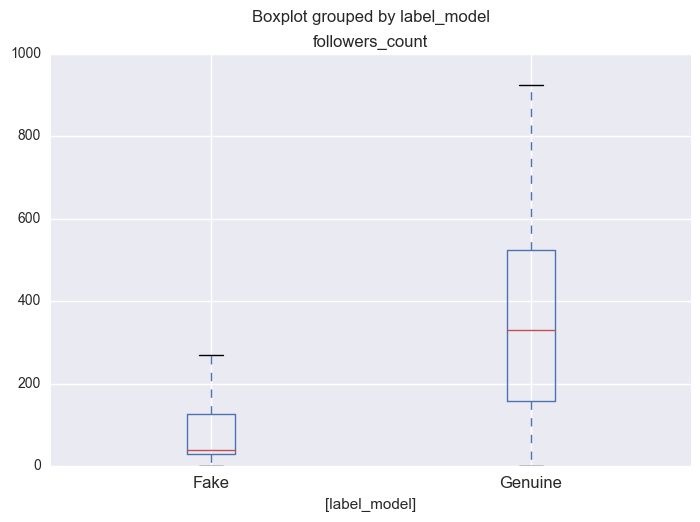
\includegraphics[width =\linewidth]{followers_count.png}
	\end{subfigure}
	~
	\begin{subfigure}[c]{0.3\linewidth}
		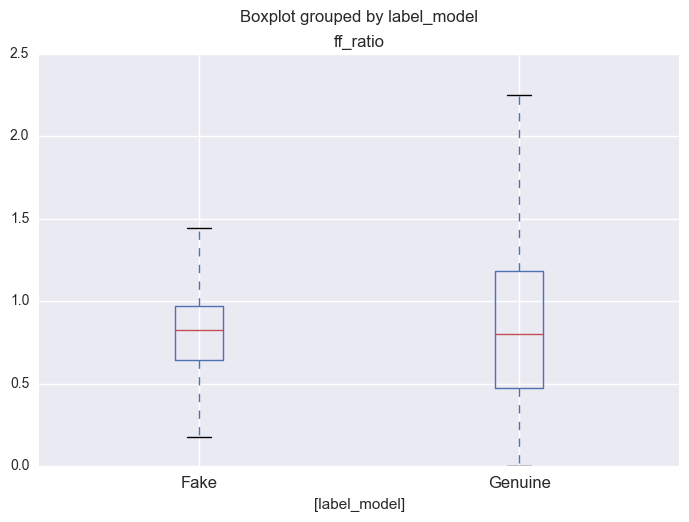
\includegraphics[width =\linewidth]{ff_ratio.png}
	\end{subfigure}
    ~
    \begin{subfigure}[c]{0.3\linewidth}
    	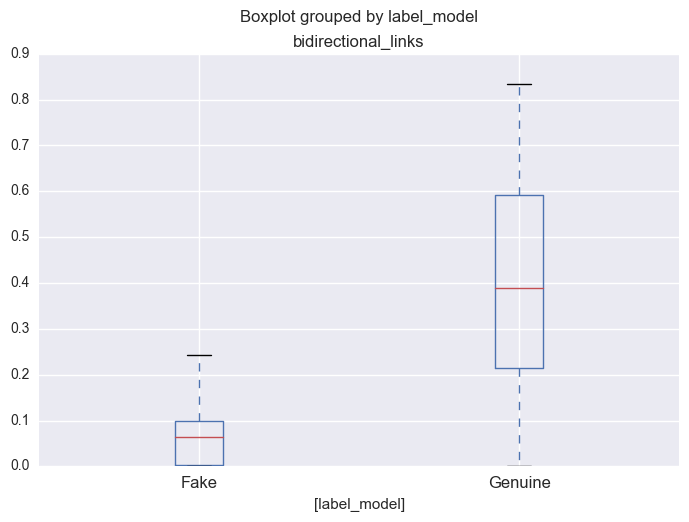
\includegraphics[width =\linewidth]{bidirectional_links.png}
    \end{subfigure}
	~
    \begin{subfigure}[c]{0.3\linewidth}
    	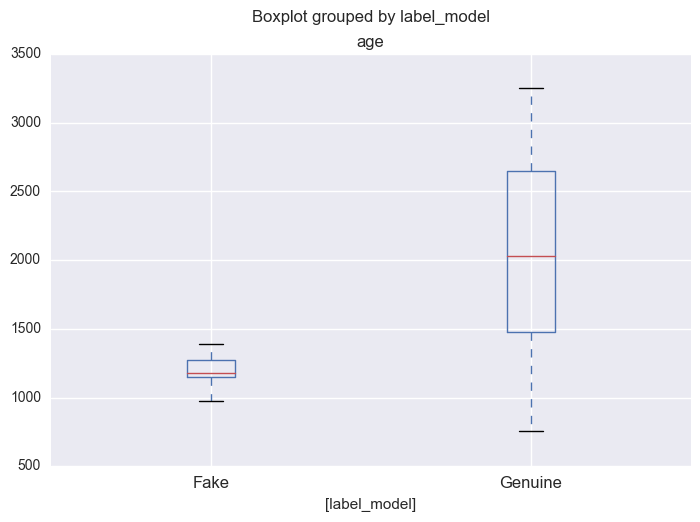
\includegraphics[width =\linewidth]{age.png}
    \end{subfigure}
	~
	\begin{subfigure}[c]{0.3\linewidth}
		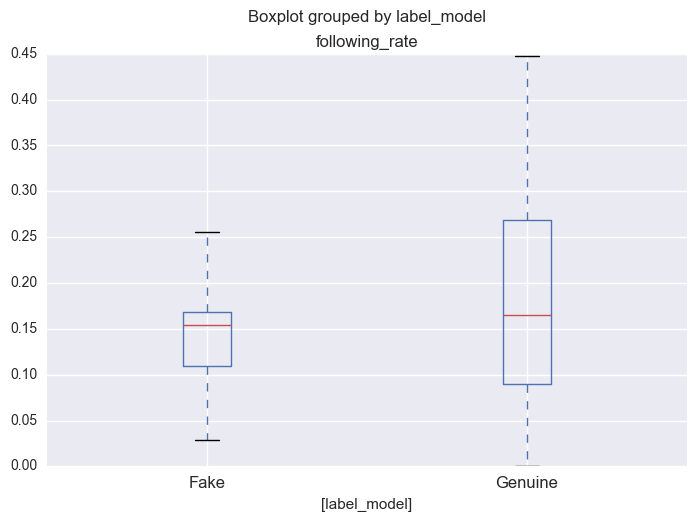
\includegraphics[width =\linewidth]{following_rate.png}
	\end{subfigure}
	~
	\begin{subfigure}[c]{0.3\linewidth}
		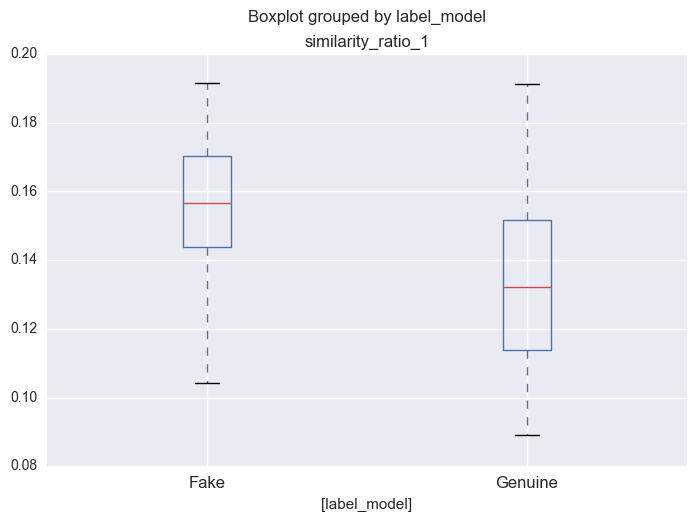
\includegraphics[width =\linewidth]{similarity_ratio_1.png}
	\end{subfigure}
	~
	\begin{subfigure}[c]{0.3\linewidth}
	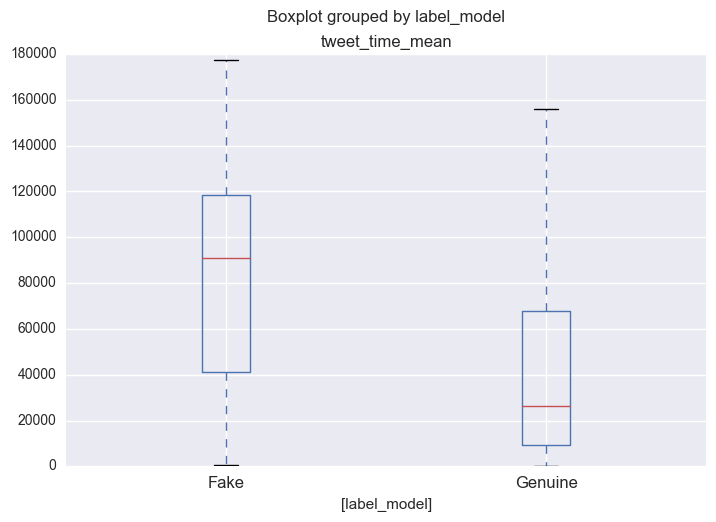
\includegraphics[width =\linewidth]{tweet_time_mean.png}
	\end{subfigure}
	~
	\begin{subfigure}[c]{0.3\linewidth}
	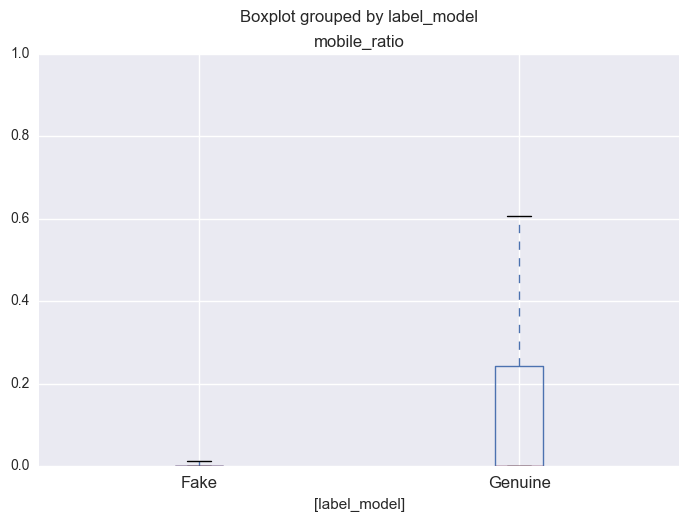
\includegraphics[width =\linewidth]{mobile_ratio.png}
	\end{subfigure}
	~
	\begin{subfigure}[c]{0.3\linewidth}
	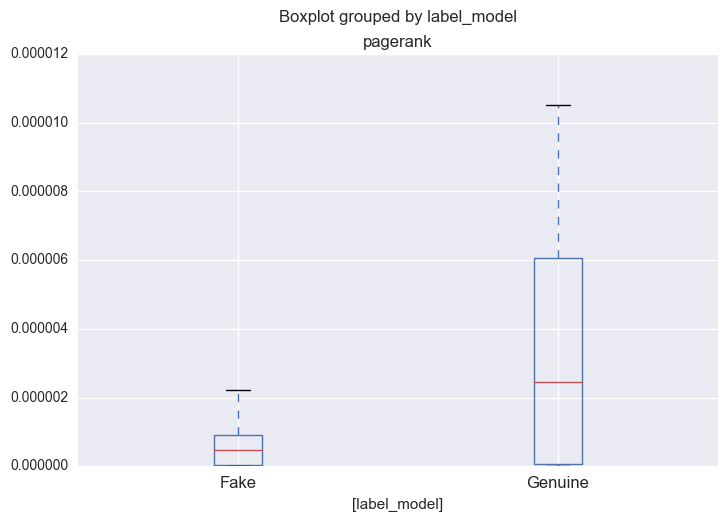
\includegraphics[width =\linewidth]{pagerank.png}
	\end{subfigure}
	\caption{Feature Boxplots of Fake Users and Genuine Users}
\end{figure}

\noindent From the above plots, we found the preliminary charactristics of fake/spam users:
\begin{enumerate}
	\item Large amount of followings in short period
	\item Less connected social relations
	\item Frequent tweeting behavior
\end{enumerate}

\subsection*{Random Forest Tree}
We applied 47 features on the randomly selected twitter accounts. Then, we use these feature scores and their appropriate labels to build a random forest. This model takes a subset of the datasets and features to build the decision trees. It repeatedly build multiple trees and aggregate the prediction results. \par

\noindent We first randomly chose 70\% of our data as training dataset and 30\% as testing dataset. In order to increase the predictive power and make it easier to train the model, we used the RandomizedSearchCV function in Scikit-learn library to find the best parameters. Table 1 shows the descriptions of the features that we believe can improve the model's performance, accuracy and speed. Table 2 displays the optimal parameters and values found from RandomizedSearchCV for all 4 sample datasets.

\begin{table}[h!]
	\caption{Parameter Descriptions}
	\begin{tabular}{ | l | p{12cm} |}
		\hline
		Parameter & Description  \\
		\hline
		max\_features & The number of features to consider when looking for the best split \\ 
		\hline
		n\_estimators & The number of trees in the forest \\ 
		\hline
		min\_samples\_leaf & The minimum number of samples required to be at a leaf node \\
		\hline
		criterion & The function that measures the quality of a split  \\
		\hline
		random\_state & The random number generator \\ 
		\hline
		class\_weight & A function that  penalizes mistakes in samples of class[i] \\ 
		\hline
	\end{tabular}
\end{table}

\begin{table}[h!]
	\caption{Best Parameters for Random Forest}
	\begin{tabular}{l*{4}{c}r}
		\hline
		Parameters     & Sample\_Data\_1 & Sample\_Data\_2 & Sample\_Data\_3 & Sample\_Data\_4 \\
		\hline
		max\_features & log2 & log2 & log2 & log2  \\
		n\_estimators & 126 & 103 & 180 & 195  \\
		min\_samples\_leaf & 69 & 50 & 69 & 52  \\
		criterion & entropy & gini & gini & gini  \\
		random\_state & 1 & 12 & 15 & 10  \\
		class\_weight & {0:10} & {0:10} & {0:10} & {0:10}  \\
		\hline
	\end{tabular}
\end{table}

\begin{table}[h!]
	\caption{Cross Validation and Accuracy Score}
	\centering
	\begin{tabular}{p{3cm} |p{3.5cm}|p{3.5cm}|p{3.5cm}}	
		\hline
		Datasets & Cross\_Validation
		Score\_Mean    & Cross\_Validation
		Score\_Standard Deviation
		& Metrics\_Accuracy
		Score\\
		\hline
		Sample\_Data\_1 & 0.942    &0.014 & 0.942\\
		\hline
		Sample\_Data\_2 & 0.961    &0.008 & 0.961\\
		\hline
		Sample\_Data\_3 & 0.964    &0.009 & 0.964\\
		\hline
		Sample\_Data\_4 & 0.913    &0.014 & 0.913\\
		\hline
	\end{tabular}
\end{table}

\noindent When tuning the parameters, we conducted 5-fold cross validation, in which allows us to randomly partition the training data into 5 equal size subsamples and evaluate the random forest model. In addition, we also find the accuracy score, in which calculates the probability that the predicted labels match with the true labels. From table 3, we can see that the cross validation scores for Sample Datasets\_1 to 3 are ranged from 0.95 and 0.98. However, the score for Sample\_Datasets\_4 is much lower than the rest. We believe the distribution of fake and genuine accounts in these datasets contribute to the difference in scores. For the first three sample datasets, we mimic the true distribution in reality, in which 10\% of them are fake and 90\% are genuine. But the ratios of sample dataset\_4 is 3:1. \par

\noindent After finding the best parameters, we used them to fit the model on the training datasets and illustrated the importance of each feature ratio in predicting the correct twitter account label with barplot. Figure 2 shows the total number of favorites that a particular user gets is the most effective predictor for sample dataset (1~3) because this feature is based on how the third party (other twitter users) responds to the content that this particular user has produced. However, if 30\% of our sample dataset are fake accounts, the website ratio has the highest predictive power because high percentage score is a good indicator of fake account.  

\begin{figure}[h!]
	\centering
	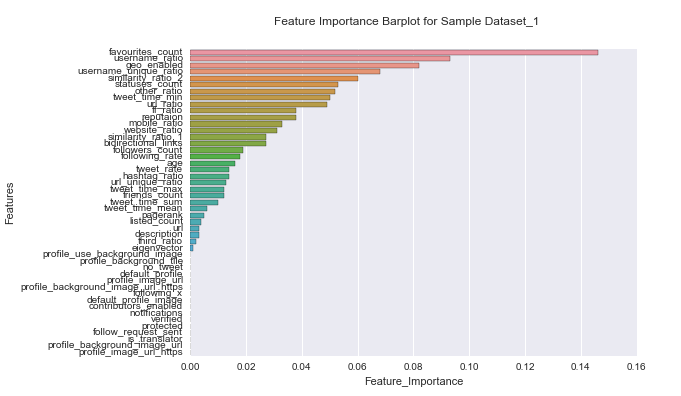
\includegraphics[scale=0.7]{feature_1}
	\caption{Feature Importance}
\end{figure}

\noindent Lastly, we used confusion matrix to check the accuracy of the random forest model. In order to better visualize and interpret the results, we used the normalized confusion matrix to make sure the ratio is at the same scale. Figure 3 and 4 show that fake accounts have higher prediction accuracy score in general, which indicates that the model did a better job in predicting fake accounts than genuine accounts. However, we also noticed that this model has a significantly higher error rate when the ratio for genuine and fake accounts is 3:1 in the dataset. 

\begin{figure}[h!]
	\centering
	\begin{subfigure}{0.45\linewidth}
		\centering
		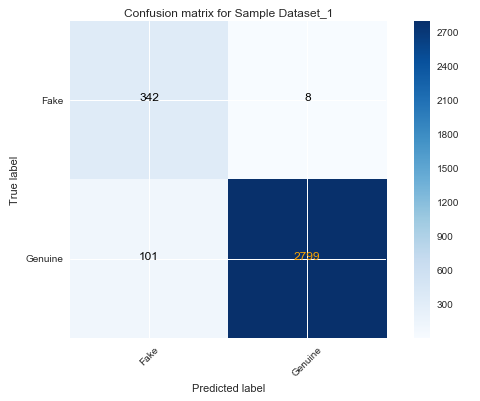
\includegraphics[width =\linewidth]{matrix_1}
		\subcaption{Without Normalization}
	\end{subfigure}%
	\begin{subfigure}{0.45\linewidth}
		\centering
		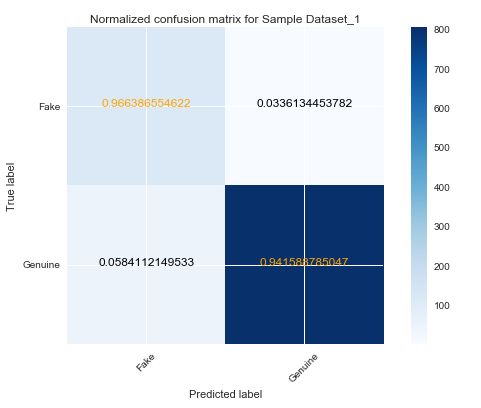
\includegraphics[width =\linewidth]{matrix_nor_1}
		\subcaption{With Normalization}
	\end{subfigure}
	\caption{Confusion Matrix for Sample 1}
\end{figure}

\begin{figure}[h!]
	\centering
	\begin{subfigure}{0.45\linewidth}
		\centering
		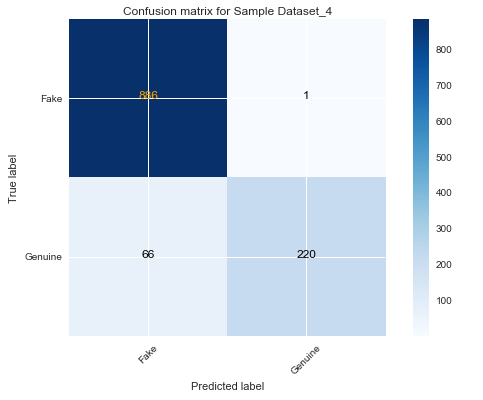
\includegraphics[width =\linewidth]{matrix_4}
		\subcaption{Without Normalization}
	\end{subfigure}%
	\begin{subfigure}{0.45\linewidth}
		\centering
		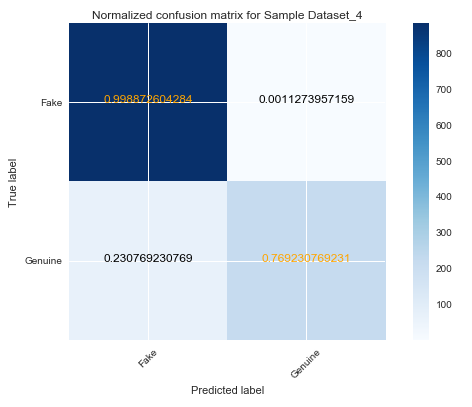
\includegraphics[width =\linewidth]{matrix_nor_4}
		\subcaption{With Normalization}
	\end{subfigure}
	\caption{Confusion Matrix for Sample 4}
\end{figure}

\subsection*{Logistic Regression}
First, we ran a default logistic model with cost parameter $C=1$, although the accuracy of identifying account by using Logistic Classification is around 90.92\%, the ratio of identifying fake account given true label is only around 35.52\%. This is because the accuracy of genuine given the true lbel improve the overall accuracy. The goal of this project is to identify the fake account accurately, even if the overall accuracy would relatively decrease a little bit.

\noindent Then we start to tune the parameters for logistic classification model by using GridSearchCV in Scikit-learn library to find the best parameters. The main parameters to tune are C, penalty and the class\_weight. The C is inverse of regularization strength which is parameter of the penalty. Also, the settings of the penalty here are L1 and L2. The most important thing we need to adjust is the class weight for the fake to penalize the error to identifying fake account.

\begin{table}[h!]
	\captionof{table}{Best Parameters of Logistic Regression} \label{tab:title} 
	\begin{center}
		\begin{tabular}{rrrrrr}
			\hline
			& Cost & Penalty & Class weight & Mean validation score & Accuracy score\\
			\hline
			Sample 1 & 1.0 & l1 & 3 & 0.964 & 0.962\\
			Sample 2 & 100 & l1 & 3 & 0.960 & 0.971\\
			Sample 3 & 10  & l1 & 3 & 0.970 & 0.965\\
			\hline
		\end{tabular}
	\end{center}
\end{table}

\noindent After getting the new parameters and fitting the new model, we gain the higher accuracy of identify accounts which is 95.38\%. Moreover, the the ratio of predicting fake account correctly is about the 88.16\%.

\subsection*{Support Vector Machine}
\subsubsection*{rbf SVM}
In rbf kernel SVM, our objective is to find the best cost parameter C, gamma $\gamma$ in kernel function and class weight which will penalize more on missclassification of fake users. After gridsearching with 5-folder cross-validation, most combination of parameters yieled the same mean validaton score. We selected one of them of each sample data as follows.

\begin{table}[h!]
	\captionof{table}{Best Parameters of rbf SVM} \label{tab:title} 
	\begin{center}
		\begin{tabular}{rrrrrr}
			\hline
			& Cost & $\gamma$ & Class weight & Mean validation score & Accuracy score\\
			\hline
			Sample 1 & 0.01 & 0.01 & 5 & 0.893 & 0.890\\
			Sample 2 & 0.01 & 0.001 & 3 & 0.969 & 0.893\\
			Sample 3 & 0.01 & 0.01 & 5 & 0.893 & 0.890\\
			\hline
		\end{tabular}
	\end{center}
\end{table}

\noindent Confusion matrix shows that all the test data is labeled as genuine, indicating that rbf SVM kernel failed to discriminate small-proportioned fake uesrs from large amount of genuine accounts. Although the general accuracy score is acceptable, the model is still useless for detection purpose.
\begin{figure}[h!]
	\centering
	\begin{subfigure}[c]{0.45\linewidth}
		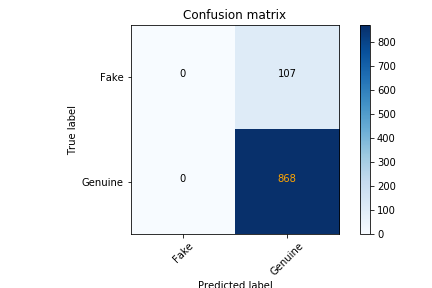
\includegraphics[width =\linewidth]{rbf_svc_confm_11.png}
	\end{subfigure}
	~
	\begin{subfigure}[c]{0.45\linewidth}
		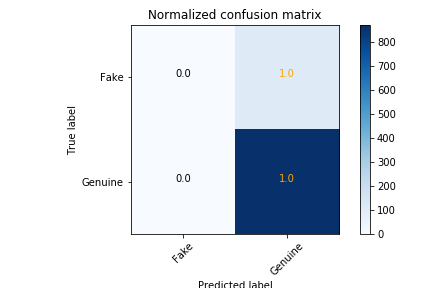
\includegraphics[width =\linewidth]{rbf_svc_confm_12.png}
	\end{subfigure}
	\caption{Confusion Matrix of rbf SVM}
\end{figure}


\subsubsection*{Linear SVM}
In linear SVM model, our objective is to find the best norm used in the penalization, cost parameter C and class weight which will penalize more on missclassification of fake users. After gridsearching with 5-folder cross-validation, we have the best set fo parameters as follows.

\begin{table}[h!]
	\captionof{table}{Best Parameters of Linear SVM} \label{tab:title} 
	\begin{center}
		\begin{tabular}{rrrrrr}
			\hline
			& Cost & Penalty & Class weight & Mean validation score & Accuracy score\\
			\hline
			Sample 1 & 100 & l1 & 3 & 0.960 & 0.960\\
			Sample 2 & 100 & l1 & 3 & 0.969 & 0.960\\
			Sample 3 & 100 & l1 & 3 & 0.968 & 0.963\\
			\hline
		\end{tabular}
	\end{center}
\end{table}

\noindent The confusion matrix of sample 3 which has the lowest TP(labeld as False user and predicted as False user) is as following. The TP rate is approximately 91\% and FP rate is approximately 3\%. Although there is a process to appeal for users who are suspended, we still want relatively low FP rate since it is possilble to lose a genuine users when it is classifed as fake account.
\begin{figure}[h!]
	\centering
	\begin{subfigure}[c]{0.45\linewidth}
		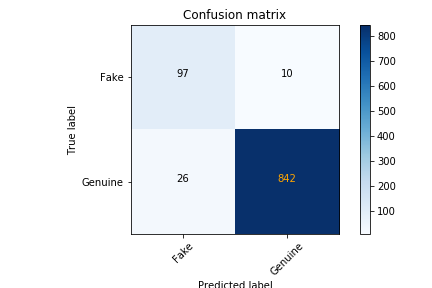
\includegraphics[width =\linewidth
		]{linear_svc_confm_31.png}
	\end{subfigure}
	~
	\begin{subfigure}[c]{0.45\linewidth}
		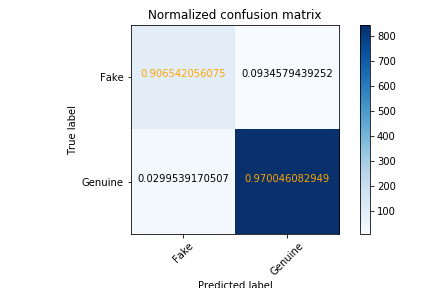
\includegraphics[width =\linewidth]{linear_svc_confm_32.png}
	\end{subfigure}
	\caption{Confusion Matrix of Linear SVM}
\end{figure}
\section*{FUTURE DISCUSSION}
Here are some possible directions that we are considering for the next step:

\noindent 1. Create more features in predicting the account type\\
2. Further evaluate the models that we built and use methods to reduce noise and errors\\
3. Investigate on other models that we can potentially use\\
4. Create an interactive platform to allow the Twitter users to use our predictive models\\

\newpage
\large\textbf{Appendix} 
\section*{Reflection}
Overall, we had successfully accomplished the goal of our project, in which allows the Twitter users to identify whether the account is fake or genuine using Random Forest, Logistic Regression and Support Vector Machine. We were unable to analyze the fake users' behaviors on the trend topics due to the time constraint. Each group member was assigned to build different features and predictive models. All of us had contributed equally. We met regularly to check on each other's progress and discuss the problems that we had encountered. Since each of us has very different levels of skill sets and knowledge, it was challenging to include and implement everyone's initial ideas. However, we were able to compromise and find common interests through discussions. Originally, we wanted to analyze all the tweets that the user has posted. However, the Twitter API has set limit on the amount of info that we could get. Therefore, we only downloaded the maximum number of tweets that we were allowed. In addition, we were planning to build features on predicting twitter account types from the scratch. However, we had realized that it is important to conduct research on previous studies and use them as references. \\

\noindent As the project progressed, we narrowed down the models that we wanted to build and try to understand the math and concepts behind them, We learned that it is important to create a feasible time-line for any project because it is often easy to overestimate the amount of work that we think we can accomplish. In addition, we need to understand the context of the data, the intuitions behind the models and how our analysis can help answer the questions that we want to solve.\\

\newpage
\section*{Plots}
\begin{figure}[h!]
	\centering
	\begin{subfigure}[c]{0.3\linewidth}
		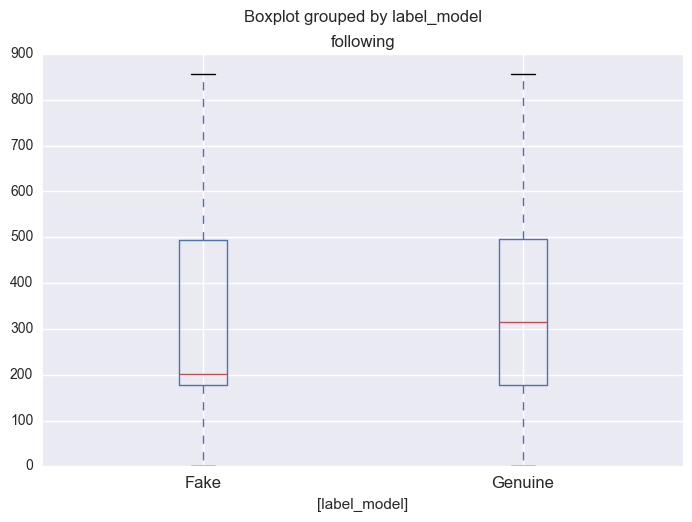
\includegraphics[width =\linewidth]{following.png}
	\end{subfigure}
	~
	\begin{subfigure}[c]{0.3\linewidth}
		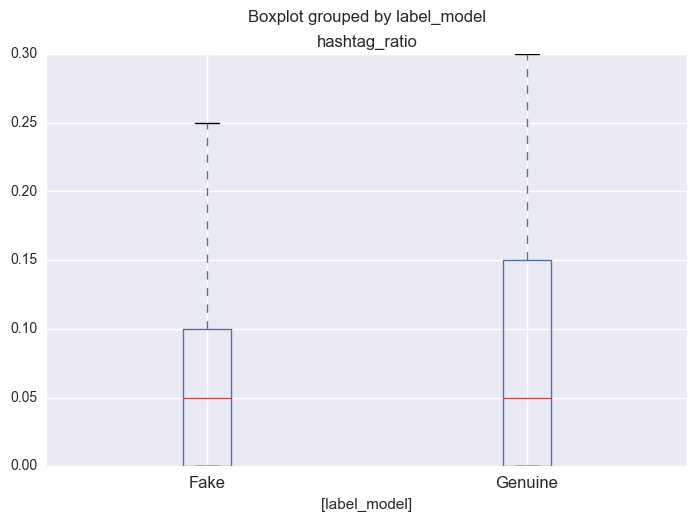
\includegraphics[width =\linewidth]{hashtag_ratio.png}
	\end{subfigure}
	~
	\begin{subfigure}[c]{0.3\linewidth}
		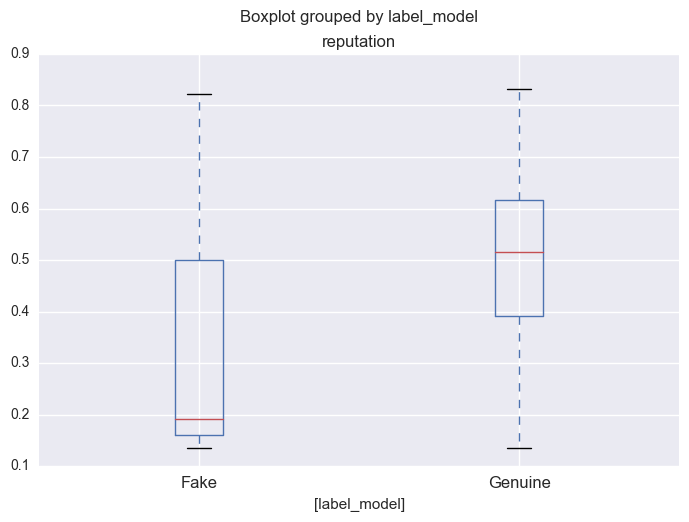
\includegraphics[width =\linewidth]{reputation.png}
	\end{subfigure}
	~
	\begin{subfigure}[c]{0.3\linewidth}
		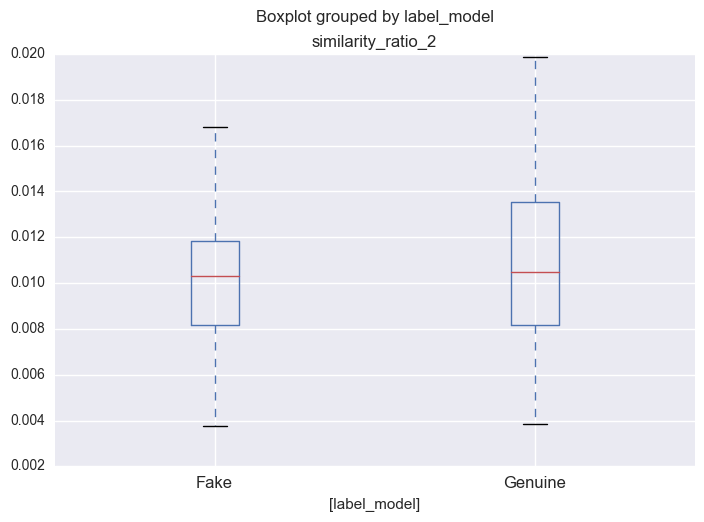
\includegraphics[width =\linewidth]{similarity_ratio_2.png}
	\end{subfigure}
	~
	\begin{subfigure}[c]{0.3\linewidth}
	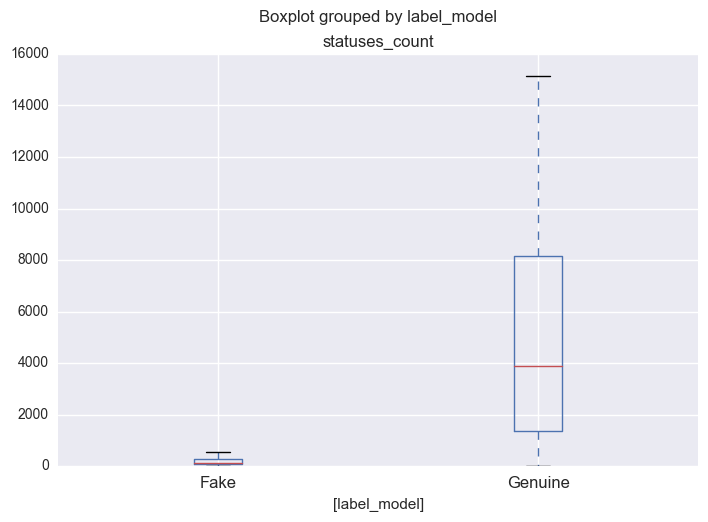
\includegraphics[width =\linewidth]{statuses_count.png}
	\end{subfigure}
	~
	\begin{subfigure}[c]{0.3\linewidth}
		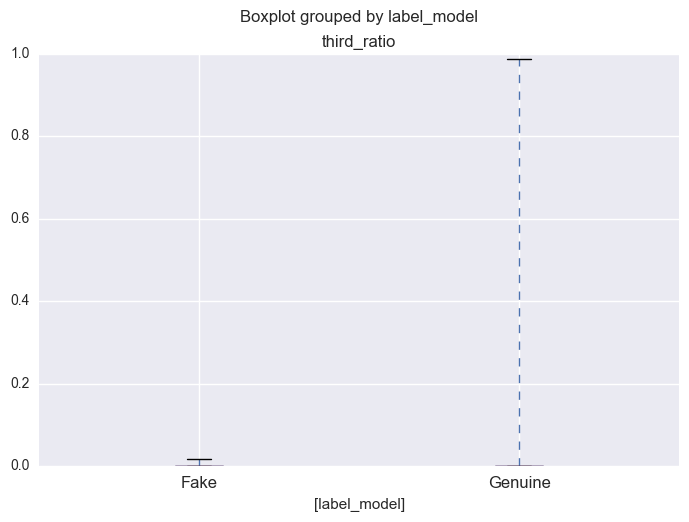
\includegraphics[width =\linewidth]{third_ratio.png}
	\end{subfigure}
	~
	\begin{subfigure}[c]{0.3\linewidth}
		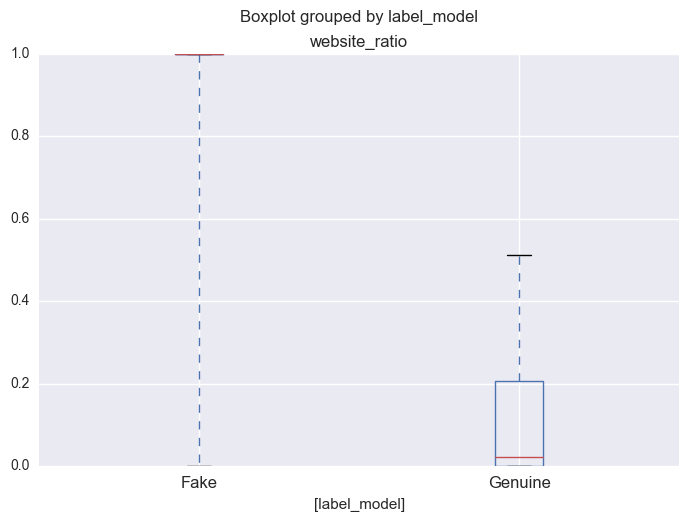
\includegraphics[width =\linewidth]{website_ratio.png}
	\end{subfigure}
	~
	\begin{subfigure}[c]{0.3\linewidth}
		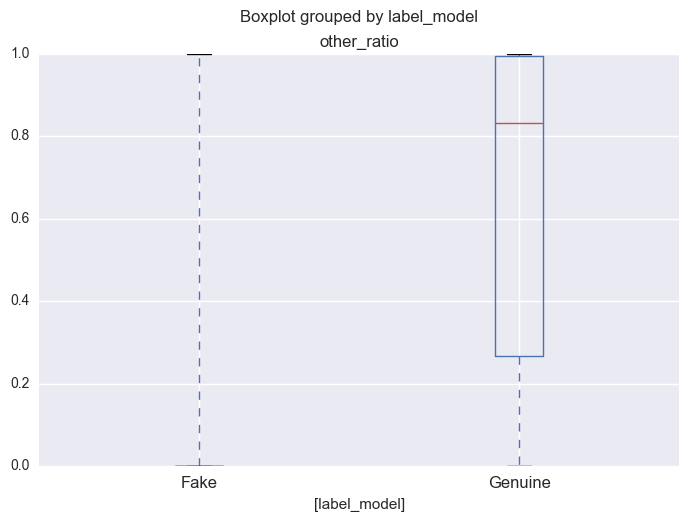
\includegraphics[width =\linewidth]{other_ratio.png}
	\end{subfigure}
	~
	\begin{subfigure}[c]{0.3\linewidth}
		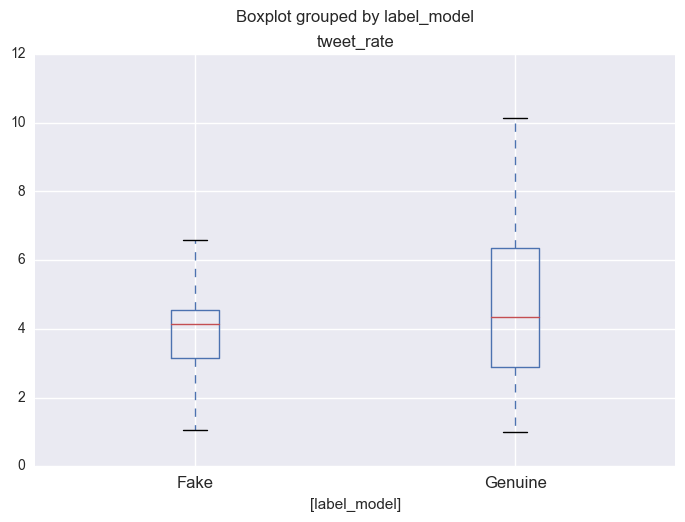
\includegraphics[width =\linewidth]{tweet_rate.png}
	\end{subfigure}
	~
	\begin{subfigure}[c]{0.3\linewidth}
		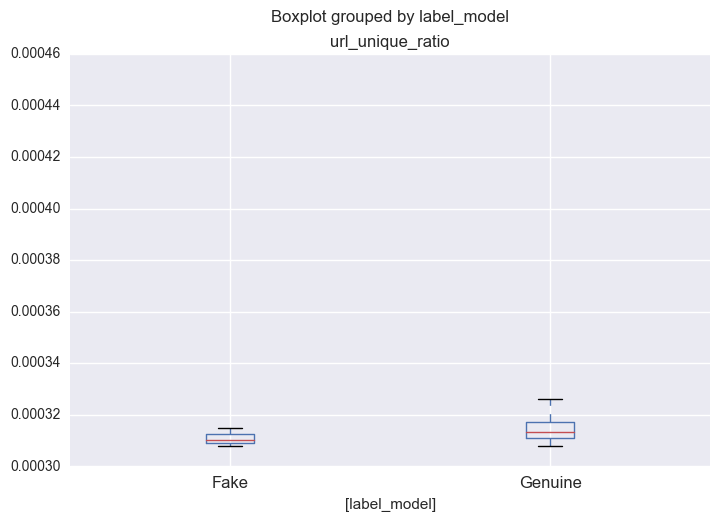
\includegraphics[width =\linewidth]{url_unique_ratio.png}
	\end{subfigure}
	~
	\begin{subfigure}[c]{0.3\linewidth}
		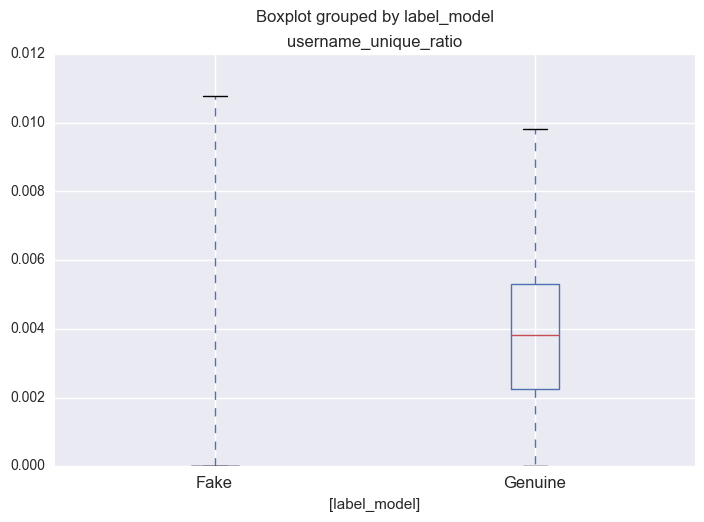
\includegraphics[width =\linewidth]{username_unique_ratio.png}
	\end{subfigure}
	\caption{Feature Comparison}
\end{figure}

\begin{figure}[h!]
	\centering
	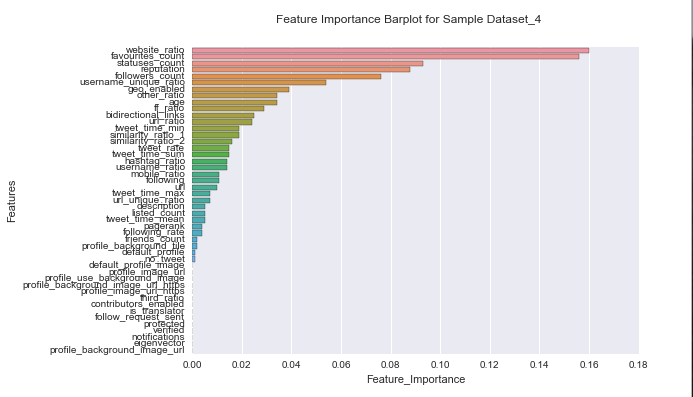
\includegraphics[scale=0.7]{feature_4}
	\caption{Feature Importance}
	\label{fig:mesh1}
\end{figure}

\newpage
\section*{Codes}
random\_forest.py - builds random forest model\\
t\_analysis.py - calculates tweet analysis ratios\\
similarity\_1.py - calculates tweet similarity ratio 1\\
similarity\_2.py - calculates tweet similarity ratio 2\\
tweet\_ratio.py - creates a csv file that contains the tweet analysis ratios\\
sim\_1\_df.py - creates a csv file for storing the tweet similarity ratio 1 result\\
sim\_2\_df.py - creates a csv file for storing the tweet similarity ratio 2 result\\
combine\_df.py - combines all the feature results into a dataframe\\
tweet\_time\_diff.py - calculates the time difference between two consecutive tweets\\


\newpage
\section*{Reference}
\begin{lstlisting}
[1]O.Varol, E.Ferrara, C.A.Davis, F.Menczer, and A.Flammini. Online Human-Bot Interactions: Detection, Estimation, and Characterization
[2] F. Benevenuto, G. Magno, T. Rodrigues, and V. Almeida. Detecting Spammers on Twitter. In Collaboration, Electronic messaging, Anti-Abuse and Spam Confference.
[3] K. Lee, J. Caverlee, and S. Webb. Uncovering Social Spammers: Social Honeypots Machine Learning. In ACM SIGIR Conference (SIGIR), 2010.
[4] G. Stringhini, S. Barbara, C. Kruegel, and G. Vigna. Detecting Spammers On Social Networks. In Annual Computer Security Applications Conference (ACSAC’10), 2010.
[5] A. Wang. Don’t follow me: spam detecting in Twitter. In Int’l Conferene on Security and Cryptography (SECRYPT), 2010.
[6] G. Stringhini, C. Kruegel, G. Vigna Detecting Spammers on Social Networks
[7] C. Yang, R. Harkreader, and G. Gu. Empirical evaluation and new design for fighting evolving Twitter spammers. I.
[8] Nando de Freitas. "Machine learning - Random forests." Online video clip. YouTube. YouTube, 21 Feb 2013
[9] https://web.stanford.edu/~jurafsky/slp3/7.pdf
 
\end{lstlisting}
\end{document} 